\documentclass[border=10pt]{standalone}
	\usepackage{amsmath}
	\usepackage{tikz}
	\usetikzlibrary{calc}


\begin{document}

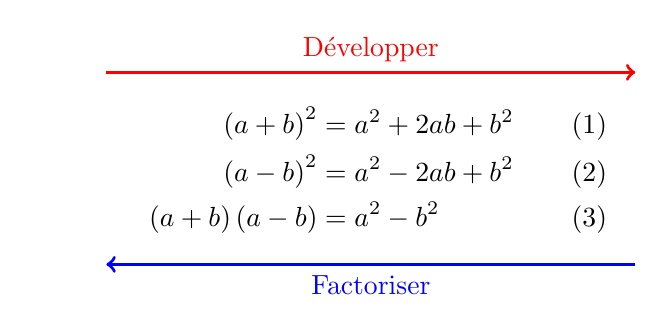
\begin{tikzpicture}
	\tikzstyle {ex}=[draw,color=white,rectangle, inner sep =10pt, inner ysep=10pt, text =black]
	\node [ex](box){%
		\begin{minipage}{7cm}\vspace{-\abovedisplayskip}%
			\begin{align}
				\left(a+b\right)^{2} & = a^{2}+2ab+b^{2}  \\
				\left(a-b\right)^{2} & = a^{2}-2ab+b^{2}   \\
				\left(a+b\right)\left(a-b\right) & = a^{2}-b^{2}
			\end{align}
		\end{minipage}
	};
	\draw[color=red,very thick,->] ($(box.north west) + (1cm,0cm)$) -- ($(box.north east) + (0cm,0cm)$)
		node[midway,above]{\textcolor{red}{D\'evelopper}};
	\draw[color=blue,very thick,->] ($(box.south east) + (0cm,0cm)$) -- ($(box.south west) + (1cm,0cm)$)
		node[midway,below]{\textcolor{blue}{Factoriser}};
\end{tikzpicture}

\end{document}